% Template for PLoS
% Version 3.5 March 2018
%
% % % % % % % % % % % % % % % % % % % % % %
%
% -- IMPORTANT NOTE
%
% This template contains comments intended 
% to minimize problems and delays during our production 
% process. Please follow the template instructions
% whenever possible.
%
% % % % % % % % % % % % % % % % % % % % % % % 
%
% Once your paper is accepted for publication, 
% PLEASE REMOVE ALL TRACKED CHANGES in this file 
% and leave only the final text of your manuscript. 
% PLOS recommends the use of latexdiff to track changes during review, as this will help to maintain a clean tex file.
% Visit https://www.ctan.org/pkg/latexdiff?lang=en for info or contact us at latex@plos.org.
%
%
% There are no restrictions on package use within the LaTeX files except that 
% no packages listed in the template may be deleted.
%
% Please do not include colors or graphics in the text.
%
% The manuscript LaTeX source should be contained within a single file (do not use \input, \externaldocument, or similar commands).
%
% % % % % % % % % % % % % % % % % % % % % % %
%
% -- FIGURES AND TABLES
%
% Please include tables/figure captions directly after the paragraph where they are first cited in the text.
%
% DO NOT INCLUDE GRAPHICS IN YOUR MANUSCRIPT
% - Figures should be uploaded separately from your manuscript file. 
% - Figures generated using LaTeX should be extracted and removed from the PDF before submission. 
% - Figures containing multiple panels/subfigures must be combined into one image file before submission.
% For figure citations, please use "Fig" instead of "Figure".
% See http://journals.plos.org/plosone/s/figures for PLOS figure guidelines.
%
% Tables should be cell-based and may not contain:
% - spacing/line breaks within cells to alter layout or alignment
% - do not nest tabular environments (no tabular environments within tabular environments)
% - no graphics or colored text (cell background color/shading OK)
% See http://journals.plos.org/plosone/s/tables for table guidelines.
%
% For tables that exceed the width of the text column, use the adjustwidth environment as illustrated in the example table in text below.
%
% % % % % % % % % % % % % % % % % % % % % % % %
%
% -- EQUATIONS, MATH SYMBOLS, SUBSCRIPTS, AND SUPERSCRIPTS
%
% IMPORTANT
% Below are a few tips to help format your equations and other special characters according to our specifications. For more tips to help reduce the possibility of formatting errors during conversion, please see our LaTeX guidelines at http://journals.plos.org/plosone/s/latex
%
% For inline equations, please be sure to include all portions of an equation in the math environment.  For example, x$^2$ is incorrect; this should be formatted as $x^2$ (or $\mathrm{x}^2$ if the romanized font is desired).
%
% Do not include text that is not math in the math environment. For example, CO2 should be written as CO\textsubscript{2} instead of CO$_2$.
%
% Please add line breaks to long display equations when possible in order to fit size of the column. 
%
% For inline equations, please do not include punctuation (commas, etc) within the math environment unless this is part of the equation.
%
% When adding superscript or subscripts outside of brackets/braces, please group using {}.  For example, change "[U(D,E,\gamma)]^2" to "{[U(D,E,\gamma)]}^2". 
%
% Do not use \cal for caligraphic font.  Instead, use \mathcal{}
%
% % % % % % % % % % % % % % % % % % % % % % % % 
%
% Please contact latex@plos.org with any questions.
%
% % % % % % % % % % % % % % % % % % % % % % % %

\documentclass[10pt,letterpaper]{article}
\usepackage[top=0.85in,left=2.75in,footskip=0.75in]{geometry}

% amsmath and amssymb packages, useful for mathematical formulas and symbols
\usepackage{amsmath,amssymb}

% Use adjustwidth environment to exceed column width (see example table in text)
\usepackage{changepage}

% Use Unicode characters when possible
\usepackage[utf8x]{inputenc}

% textcomp package and marvosym package for additional characters
\usepackage{textcomp,marvosym}

% cite package, to clean up citations in the main text. Do not remove.
\usepackage{cite}

% Use nameref to cite supporting information files (see Supporting Information section for more info)
\usepackage{nameref,hyperref}

% line numbers
\usepackage[right]{lineno}

% ligatures disabled
\usepackage{microtype}
\DisableLigatures[f]{encoding = *, family = * }

% color can be used to apply background shading to table cells only
\usepackage[table]{xcolor}

% array package and thick rules for tables
\usepackage{array}

% create "+" rule type for thick vertical lines
\newcolumntype{+}{!{\vrule width 2pt}}

% create \thickcline for thick horizontal lines of variable length
\newlength\savedwidth
\newcommand\thickcline[1]{%
  \noalign{\global\savedwidth\arrayrulewidth\global\arrayrulewidth 2pt}%
  \cline{#1}%
  \noalign{\vskip\arrayrulewidth}%
  \noalign{\global\arrayrulewidth\savedwidth}%
}

% \thickhline command for thick horizontal lines that span the table
\newcommand\thickhline{\noalign{\global\savedwidth\arrayrulewidth\global\arrayrulewidth 2pt}%
\hline
\noalign{\global\arrayrulewidth\savedwidth}}


% Remove comment for double spacing
%\usepackage{setspace} 
%\doublespacing

% Text layout
\raggedright
\setlength{\parindent}{0.5cm}
\textwidth 5.25in 
\textheight 8.75in

% Bold the 'Figure #' in the caption and separate it from the title/caption with a period
% Captions will be left justified
\usepackage[aboveskip=1pt,labelfont=bf,labelsep=period,justification=raggedright,singlelinecheck=off]{caption}
\renewcommand{\figurename}{Fig}

% Use the PLoS provided BiBTeX style
\bibliographystyle{plos2015}

% Remove brackets from numbering in List of References
\makeatletter
\renewcommand{\@biblabel}[1]{\quad#1.}
\makeatother



% Header and Footer with logo
\usepackage{lastpage,fancyhdr,graphicx}
\usepackage{epstopdf}
%\pagestyle{myheadings}
\pagestyle{fancy}
\fancyhf{}
%\setlength{\headheight}{27.023pt}
%\lhead{\includegraphics[width=2.0in]{PLOS-submission.eps}}
\rfoot{\thepage/\pageref{LastPage}}
\renewcommand{\headrulewidth}{0pt}
\renewcommand{\footrule}{\hrule height 2pt \vspace{2mm}}
\fancyheadoffset[L]{2.25in}
\fancyfootoffset[L]{2.25in}
\lfoot{\today}

%% Include all macros below

\newcommand{\lorem}{{\bf LOREM}}
\newcommand{\ipsum}{{\bf IPSUM}}

%% END MACROS SECTION


%%%%%%PACKAGES
\usepackage{graphicx}
\graphicspath{{images/}}

\usepackage{tikz}
\usetikzlibrary{shapes.geometric, arrows}
\tikzstyle{mainNode} = [rectangle, rounded corners, minimum width=3cm, text width=6cm, minimum height=1cm,text centered, draw=black]
\tikzstyle{branchNode} = [rectangle, rounded corners, minimum width=3cm, text width=4cm, minimum height=1cm,text centered, draw=black]
\tikzstyle{arrow} = [thick,->,>=stealth]

\usepackage{color}

\usepackage{hyperref}
\hypersetup{
        colorlinks=true,
        linkcolor=blue,
        citecolor=blue,
        filecolor=blue,
        urlcolor=blue,
}
\urlstyle{same}

%%%%%% AUTHORS SETTINGS
\usepackage{multirow}
\usepackage{color, colortbl}
\definecolor{gray}{gray}{0.9}
\definecolor{teal}{RGB}{0, 120, 120}
\definecolor{brickred}{RGB}{199, 59, 55}
% \usepackage{indentfirst}
\usepackage{array}
\usepackage{enumitem}
\usepackage{caption}
\usepackage{amsmath}
\usepackage{multicol}

% \setcounter{secnumdepth}{4}
\newcolumntype{g}{>{\small\columncolor{gray}}c}
\newcolumntype{x}{>{\small\columncolor{gray}}l}
\newcolumntype{C}{>{\small}c}
\newcolumntype{V}{>{\footnotesize}c}
\newcolumntype{L}[1]{>{\small}l{#1}}
\newcolumntype{P}[1]{>{\small}p{#1}}
\newcommand{\myparagraph}[1]{\paragraph*{#1}\mbox{}\\}
\newcommand{\tbm}[1]{\color{teal} {\begin{itemize} \item {\footnotesize #1} \end{itemize}}  \normalsize \color{black}}
\newcommand{\TG}[1]{\color{blue}From Tristan: #1\\ \color{black}}
\newcommand{\GK}[1]{\color{blue}From Greg: #1\\ \color{black}}
\newcommand{\git}[1]{\href{https://github.com/big-data-lab-team/reproducibility-bioinfo/#1}}
\newcommand{\svm}{\href{http://svmlight.joachims.org}}
\newcommand{\trssp}[1]{\href{http://bioinfo.noble.org/TrSSP/#1}}
\newcommand{\ncbi}[1]{\href{https://www.ncbi.nlm.nih.gov/#1}}
\newcommand{\pa}[1]{\small{#1}\normalsize}
\newcommand{\mrko}[1]{\color{brickred}{#1}\color{black}}
\newcommand{\mrkm}[5]{
        \color{brickred}{#1}&\color{brickred}{#2}&
        \color{brickred}{#3}&\color{brickred}{#4}&
        \color{brickred}{#5} \color{black}}
\newcommand{\tabitem}[1]{\item[--]{\footnotesize{#1}}}
\newcommand{\refitem}[1]{\item[]{\footnotesize{#1}}}

\begin{document}
\vspace*{0.2in}

% Title must be 250 characters or less.
\begin{flushleft}
{\Large
\textbf\newline{Membrane Protein Classification: a Reproducibility Study} % Please use "sentence case" for title and headings (capitalize only the first word in a title (or heading), the first word in a subtitle (or subheading), and any proper nouns).
}
\newline
% Insert author names, affiliations and corresponding author email (do not include titles, positions, or degrees).
\\
Hamidreza Heidarzadeh,
Gregory Kiar,
Tristan Glatard
\\
\bigskip
Department of Computer Science and Software Engineering, Concordia University, Montreal, Quebec, Canada
\bigskip

% Insert additional author notes using the symbols described below. Insert symbol callouts after author names as necessary.


% Current address notes
% \textcurrency Current Address: Dept/Program/Center, Institution Name, City, State, Country % change symbol to "\textcurrency a" if more than one current address note
% \textcurrency b Insert second current address 
% \textcurrency c Insert third current address

\end{flushleft}
% Please keep the abstract below 300 words
\section*{Abstract}
Abstract goes here


% Please keep the Author Summary between 150 and 200 words
% Use first person. PLOS ONE authors please skip this step. 
% Author Summary not valid for PLOS ONE submissions.   
% \section*{Author summary}
% Author summary goes here

\linenumbers

\section {Introduction}

\TG{Add a sentence starting with ``The goal of this paper is \ldots''}
\tbm{FAIR: Finable, Accessible, Interoperable, Reusable}
\tbm{Joelle Pineau:  Machine Learning Reproducibility Checklist}
\tbm{Plos One: Ten Simple Rules for Reproducible Computational Research}

\tbm{We picked a paper with Imbalanced dataset problem}
Reproducible results are an essential requirement for computational studies including those based on machine learning techniques. 
Researchers' studies are often based on previously published experiments being conducted by their team or other scientists 
through the same field of study. 
Throughout the process, they may apply a new computational technique or a new model to the problem, 
approach the same problem from a different perspective or add up their own contribution to the field. \\

Failing to achieve the based results after reproducing a reported experiment, can cause significant financial costs 
and loss of time depending on the conducted study. The problem can be often addressed either through running the same 
experiment in an environment different than the original one (caused by changes in technology and tools available to a 
researcher at the time the study was conducted) or failing to report some details which may not look important but 
can significantly affect the reproduced results. \\

The solution for this common problem is sharing the work's dataset, features, source code and dependencies with other 
researchers using available means. Considering the fact that this may not be possible all the time, we need to make 
sure to report on all the details involved in the process. Through this work, we conducted a reproducibility study on a paper 
in bio-informatics field to address the missing details that could affect the reproduced results and create a guideline for 
having a reproducible experiment.\\

The diagram in Section~\ref{sec:supporingMaterials} illustrates the process through which our study was conducted. The code base for 
this paper is available at the paper's \git{}{GitHub} repository.

\section{Materials and Methods}

    \subsection{Dataset}   

    The dataset contains 780 transporter proteins classified into 7 substrate specific classes (70 amino acid transporters, 
    60 anion transporters, 260 cation transporters, 60 electron transporters, 70 protein/mRNA transporters, 60 sugar 
    transporters, 200 other transporters) and one none-transporter class (600 proteins) for a total of 1,380 protein 
    sequences which are available at  \trssp{?dowhat=Datasets}{TrSSP} website.
    
    For the purpose of our study, we coded a program (\git{download.py}{download.py}) to download all the sequences from the 
    \ncbi{protein}{NCBI} database using the sequence accession number from TrSSP website. 
    Considering the fact that some sequences could be updated through time, we checked all the \git{dataset/trainTest/}{downloaded ones} 
    against the originals to make sure all of our sequences match those of the TrSSP. We then updated the 
    modified sequences and their accession numbers accordingly.

    \subsection{Feature extraction}

    The authors \cite{mishra2014prediction} have extracted five features out of the dataset sequences. They have then built-up different Support Vector Machine based 
    computational models using a combination of these features. Following the descriptions from the paper, we generated all the 
    \git{features/}{features} in Comma Separated Values (.csv) format adding one more column for the labels.

    Table \ref{tab:table1} in the original paper, compares different models based on 4 evaluation metrics (Sensitivity, Specificity, Accuracy and MCC) for 
    "all seven substrate-specific transporter classes". Also, under "Data Compilation" section, it has been mentioned that the five-fold 
    cross-validation has been applied to "1,380 proteins in the main dataset" that is the total number of sequences available across 
    all 8-classes being put together.

    So, to clear up any doubts, for each feature we generated the ".csv" file for both 7-class (all seven transporter classes) and 8-class 
    (all seven classes plus non-transporters) based models using \git{extractFeature.py}{extractFeature.py} program.
    
    
    \myparagraph{\small Amino Acid Composition (AAC)}
    The Amino Acid (Monopeptide) Composition is the number of amino acids of each type normalized with the total number of 
    residues \cite{gromiha2010protein}. The percentage of each amino acid was calculated using the following formula:
    \begin{equation}
        \text{percentage of amino acid (i)} = \frac {\text{total number of amino acid (i)}} {\text{total number of amino acids in protein}} * 100
    \end{equation}
    where i represents one of the 20 standard amino acids \cite{mishra2014prediction} 
    
    \myparagraph{\small Dipeptide Composition (DPC)}
    The composition of dipeptides is a measure to quantify the preference of amino acid residue pairs in a sequence 
    \cite{gromiha2010protein}. The percentage of each dipeptide is calculated using following formula where i 
    can be any dipeptide of 400 possible dipeptides. \cite{mishra2014prediction}:
    \begin{equation}
        \text{percentage of dipeptide (i)} = \frac {\text{total number of dipeptide (i)}} {\text{total number of dipeptides in protein}} * 100
    \end{equation}

    \subsection{Construction of the main dataset}
        \myparagraph{5-Fold Cross-Validation on a shuffled dataset}
        \myparagraph{5-Fold Cross-Validation out of each class}
        \myparagraph{Subsampling}

    \subsection{Class definitions}
        \myparagraph{\small 7-class-based model}
        \myparagraph{\small 8-class-based model}

    \subsection{Classifier}
        \myparagraph{Gamma and Cost}
        \myparagraph{Thresholding}

    \subsection{Evaluation}
        \myparagraph{Metrics from the paper}
        \myparagraph{Micro vs Macro}
        \myparagraph{SVM-Light vs Scikit-Learn}
\section {Results}
\label{sec:results}

In this work, we experimented on 3 software programs (SvmLight binary classifier, ScikitLearn binary classifier 
(which provides probabilities for each data point after classification) and ScikitLearn predictor 
(which classifies data point, aggregates the results and provides a final predicted label for each element)) 
for performing classification through the settings described in the section~\ref{sec:materials}. 
We experimented on datasets with 7 and 8 classes of sequences through shuffled, balanced and downsampled settings. 
The study also includes results from Micro and Macro averaging techniques through 3 different aggregation methodology 
for final label prediction.

Table \ref{tab:table1} shows the average accuracy, sensitivity, specificity and Mathews correlation coefficient values 
for amino acid composition (AAC) for models with 7 and 8 classes in their dataset when results are classified and predicted 
using ScikitLearn predictor program. Table \ref{tab:table4} and Table \ref{tab:table5} on the other hand, 
shows the average accuracy, sensitivity, specificity and Mathews correlation coefficient values for amino acid composition (AAC) 
for models with 7 (Table 2) and 8 (Table 3) classes in their dataset when results are classified using SvmLight 
and ScikitLearn binary classifiers programs.

Overall, models with 8 classes of protein sequences in the dataset perform better and provide higher numerical values 
compared to the ones with 7 classes of proteins in the dataset. The 8-class based datasets contain more sequences and 
thus there are more data available for the classification algorithm to learn from which leads to better performance results.

Regrading the different aggregation techniques, the vote-based models corresponds to multi-class classification 
problems where there is one predicted label for each element in the dataset. For the problems in this category, 
the results from all 3 software programs are very close through the same settings. We suggest the ScikitLearn predictor 
since it involves less coding and thus provides better reproducibility when merged with other tools from the ScikitLearn Library.

The class-based and threshold-based models correspond to the multi-label classification problems where there can 
be more than one predicted label for an element of the dataset. The difference is that, on class-based aggregation technique, 
the specificity-sensitivity value pairs, initially show a considerable difference(the difference amount depends on 
the software used for classification), wherein threshold-based technique we need to apply a threshold to 
the predicted results to put the specificity-sensitivity value pairs in balance.

Overall for both SvmLight and ScikitLearn binary classifiers, the closest results to the original ones are achieved through 
threshold-based aggregation technique on shuffled and balanced datasets when the metrics are Micro averaged.

ScikitLearn predictor program could not be used for class-based and threshold-based aggregation techniques because 
it aggregates and provides one label result for each element. If you want to use ScikitLearn support vector machine 
classier for these models (which is the case for problems like the work in~\cite{mishra2014prediction}) 
you need to use it as a binary classifier that provides the probability for each point and you can manage the 
aggregation technique on your own depending on the problem requirements (Table 2 and 3, ScikitLearn binary classifier).

Regarding the 2 different settings for Gamma and Cost values, compared to applying on single value pair to all classes 
of the dataset, applying different value pairs to each involved class, increases the chance of obtaining more true 
positives and thus better results. But through this work, we didn’t observe a considerable difference in between the 
results through any of those 2 settings mentioned above.

Regarding Micro versus Macro averaging techniques, Micro averaging provides higher MCC values and less difference in between 
sensitivity and specificity for almost all the models but it does not affect the accuracy greatly. Also, for balanced 
datasets (down-sampled instance), although using different averaging techniques affects the results but the impact 
is not as much as it is for imbalanced instances of the datasets (shuffled and balanced).

Regarding different instances of the dataset, the performance metric results of the balanced and shuffled 
instances of the dataset are close, where for down-sampled version of the dataset we observed lower 
values for performance metrics since compared to the balanced and shuffled instances, the down-sampled version 
contains less proteins sequences which mean less data for training the classifier.


Figure~\ref{fig:figure7} and Figur ~\ref{fig:figure8} are the specificity-sensitivity contour density plot of all 
the models built on datasets containing 7 (figure 1) and 8 (figure 2) classes of proteins. The results fit themselves 
into 3 different groups. 

The first group include the data points with the least distance to the initial results which are the results being 
achieved using threshold-based aggregation technique classified by either SvmLight or ScikitLearn binary classifiers. 
The Micro averaged results appear closer to the initial results where the Macro averaged ones appear farther but 
still in the same group. For 8 class based models (figure 8), closest results appear a bit farther from the initial 
results because they provide better results (higher values) compared to the same models with 7 protein classes 
in the dataset.

The second group above the first one on the top, corresponds to the models with class-based aggregation technique when classified 
using ScikitLearn binary classifier. The observed difference in between specificity and sensitivity values in these models 
(compared to same models when classified using SvmLight program) is probably the product of the default threshold value 
of the classifier. This group in figure 8 still appear on the top left but not completely separated from the next group as their 
performance metric values does not differ greatly from the next group. 
The third group in between these two, corresponds to all the other models of the experiment.

Table \ref{tab:table6} shows the average accuracy, sensitivity, specificity and Mathews correlation coefficient values 
from our best model setting being applied to all the features being mentioned in the table 1 of the 
initial study~\cite{mishra2014prediction}.

% Figure 1
\begin{figure}
    \begin{small}
        \begin{center}
            \includegraphics[width=0.8\textwidth]{figures/fig71}
        \end{center}
        \caption{Models with 7 classes of proteins in the dataset}
        \label{fig:figure7}
    \end{small}
\end{figure}

% Figure 2
\begin{figure}
    \begin{small}
        \begin{center}
            \includegraphics[width=0.8\textwidth]{figures/fig81}
        \end{center}
        \caption{Models with 8 classes of proteins in the dataset}
        \label{fig:figure}
    \end{small}
\end{figure}

% Table 1
\begin{table}[ht]
    \centering
    \begin{tabular}{|L || C C | C C |}
        \hline
        \rowcolor{gray}  Amino Acid Composition (AAC) &
        Accuracy  &  MCC & Gamma & Cost
        \\
        \hline \hline
        Original Results & 73.74 & 0.46 & 1-e-5 to 10 & 1 to 4\\
        \hline
        \multicolumn{5}{|x|} {7 class based models}\\
        \hline
        dataset & 18.33 & 0.03 & 0.02 & 5.0\\
        dataset (shuffled) & 45.51 & 0.29 & 0.02 & 4.6\\
        dataset (down-sampled) & 43.80 & 0.34 & 0.02 & 4.5\\
        \hline
        \multicolumn{5}{|x|} {8 class based models}\\
        \hline
        dataset & 39.05 & 0.05 & 0.02 & 4.1\\
        dataset (shuffled) & 53.76 & 0.34 & 0.02 & 4.1\\
        dataset (down-sampled) & 38.54 & 0.29 & 0.02 & 4.1\\
        \hline

    \end{tabular}
    \captionsetup{font=small,width=10cm}
    \caption{The average accuracy and MCC values for basic scikit-learn based 
    models for amino acid composition (AAC).}
    \label{tab:table1}
    
\end{table}

\begin{table}[ht]
    \centering
    \begin{tabular}{|L | V |V V V V g g g V V V V | V |}
        \hline
        \multicolumn{14}{|g|}{7-class based model for AAC}\\
        \hline
        \multicolumn{1}{|l|}{\multirow{2}{*}{\footnotesize{Original Results}}}
        &
        \multicolumn{3}{g}{Accuracy} & \multicolumn{3}{g}{Sensitivity} &
        \multicolumn{3}{g}{Specificity} & \multicolumn{4}{g|}{MCC}\\
        \cline{2-14}&
        \multicolumn{3}{C}{73.74} & \multicolumn{3}{C}{74.65} &
        \multicolumn{3}{C}{73.22} & \multicolumn{4}{C|}{0.46} \\
        \hline\hline
        
        \multicolumn{14}{|g|} {SVM Light}\\
        \hline\hline
        
        \cline{1-12}\multicolumn{1}{|g}{}&
        
        \multicolumn{1}{|g|}{\footnotesize{Dist}}&
        \multicolumn{4}{g} {\footnotesize{Gamma-Cost different for each class}}&
        \multicolumn{3}{g}{}&
        \multicolumn{4}{g|} {\footnotesize{same Gamma-Cost for all classes}}&
        \multicolumn{1}{g|}{\footnotesize{Dist}}\\
        
        \cline{3-6}\cline{10-13}\multicolumn{1}{|g}{}&
        \multicolumn{1}{|g|}{\footnotesize{ance}}&
        \multicolumn{1}{g}{acc}&\multicolumn{1}{g}{sens}&
        \multicolumn{1}{g}{spec}&\multicolumn{1}{g}{mcc}&
        \multicolumn{3}{g}{}&
        \multicolumn{1}{g}{acc}&\multicolumn{1}{g}{sens}&
        \multicolumn{1}{g}{spec}&\multicolumn{1}{g|}{mcc}&\multicolumn{1}{g|}{\footnotesize{ance}}\\

        \hline

        \multicolumn{1}{|l|}{\multirow{6}{*}{\footnotesize{Class-based}}}
        
        & 0.25 & 82.28 & 56.53 & 86.58 & 0.37 &    n&&n                & 80.73 & 60.00 & 84.18 & 0.37 & 0.21 \\
        & 0.43 & 84.07 & 39.28 & 91.55 & 0.32 &    d&\small{Micro}&d   & 81.90 & 48.33 & 87.5 & 0.32 & 0.33 \\
        & 0.26 & 81.74 & 54.74 & 86.24 & 0.36 &    sh&&sh              & 80.42 & 59.61 & 83.88 & 0.36 & 0.21 \\
        
        \cline{2-5}\cline{7-9}\cline{11-14}
        
        & 0.37 & 82.28 & 43.76 & 84.31 & 0.31 &    n&&n                & 80.73 & 46.64 & 81.69 & 0.30 & 0.33 \\
        & 0.43 & 84.08 & 39.28 & 91.54 & 0.32 &    d&\small{Macro}&d   & 81.90 & 48.33 & 87.49 & 0.33 & 0.33 \\
        & 0.38 & 81.73 & 43.27 & 84.06 & 0.28 &    sh&&sh              & 80.42 & 46.96 & 81.49 & 0.29 & 0.33 \\
        
        \hline
        \multicolumn{1}{|l|}{\multirow{6}{*}{\footnotesize{Threshold-based}}}

        &\mrkm{0.09}{73.84}{75.25}{73.60}{0.36} &    n&&n                & \mrkm{74.10}{75.12}{73.93}{0.36}{0.09} \\
        & 0.18 & 69.45 & 70.00 & 69.36 & 0.28 &     d&\small{Micro}&d   & 69.96 & 71.19 & 69.76 & 0.29 & 0.16 \\
        & 0.11 & 72.06 & 76.15 & 71.39 & 0.34 &    sh&&sh              & 72.91 & 75.38 & 72.50 & 0.35 & 0.13 \\
        
        \cline{2-5}\cline{7-9}\cline{11-14}

        & 0.20 & 73.84 & 64.18 & 70.45 & 0.28 &    n&&n                & 74.10 & 63.42 & 70.70 & 0.28 &  0.21 \\
        & 0.18 & 69.45 & 70.00 & 69.36 & 0.28 &     d&\small{Macro}&d   & 69.96 & 71.19 & 69.76 & 0.30 & 0.16 \\
        & 0.20 & 72.06 & 66.89 & 68.16 & 0.27 &     sh&&sh              & 72.91 & 64.46 & 69.24 & 0.26 & 0.21 \\
        
        \hline
        \multicolumn{1}{|l|}{\multirow{6}{*}{\footnotesize{Vote-based}}}

        & 0.35 & 84.87 & 47.05 & 91.17 & \mrko{0.38} &    n&&n                & 84.54 & 45.89 & 90.98 & 0.36 & 0.36 \\
        & 0.37 & 84.35 & 45.24 & 90.87 & 0.36 &    d&\small{Micro}&d   & 83.87 & 43.57 & 90.59 & 0.34 & 0.38 \\
        & 0.37 & 84.32 & 45.12 & 90.85 & 0.35 &    sh&&sh              & 84.21 & 44.74 & 90.79 & 0.35 & 0.37 \\
        
        \cline{2-5}\cline{7-9}\cline{11-14}

        & 0.48 & 84.87 & 34.05 & 89.58 & 0.28 &    n&&n                & 84.54 & 33.59 & 89.48 & 0.27 & 0.49 \\
        & 0.37 & 84.35 & 45.23 & 90.87 & 0.34 &    d&\small{Macro}&d   & 83.87 & 43.57 & 90.59 & 0.33 & 0.39 \\
        & 0.48 & 84.32 & 33.52 & 89.14 & 0.27 &    sh&&sh              & 84.21 & 33.47 & 89.15 & 0.27 & 0.48 \\
        
        \hline\hline
        
        \multicolumn{14}{|g|} {Scikit Learn}\\
        \hline\hline

        \multicolumn{1}{|l|}{\multirow{6}{*}{\footnotesize{Class-based}}}
        
        & 0.61 & 87.51 & 21.47 & 98.44 & 0.33 &    n&&n                 & 87.45 & 19.39 & 98.69 & 0.32 & 0.63 \\
        & 0.65 & 87.03 & 17.43 & 98.60 & 0.29 &    d&\small{Micro}&d   & 86.68 & 15.28 & 98.56 & 0.27 & 0.68 \\
        & 0.61 & 87.49 & 21.66 & 98.41 & 0.34 &    sh&&sh              & 87.55 & 20.878 & 98.63 & 0.34 & 0.62 \\
        
        \cline{2-5}\cline{7-9}\cline{11-14}
        
        & 0.66 & 87.49 & 18.29 & 98.20 & 0.24 &    n&&n                 & 87.44 & 14.87 & 98.46 & 0.20 & 0.71 \\
        & 0.67 & 87.03 & 17.46 & 98.61 & 0.24 &    d&\small{Macro}&d   & 86.68 & 15.32 & 98.56 & 0.22 & 0.70 \\
        & 0.67 & 87.47 & 17.52 & 98.18 & 0.23 &    sh&&sh              & 87.53 & 16.32 & 98.40 & 0.21 & 0.69 \\
        
        \hline
        \multicolumn{1}{|l|}{\multirow{6}{*}{\footnotesize{Threshold-based}}}
        
        & \mrkm{0.07}{75.33}{76.42}{75.13}{0.38} &    n&&n                 & \mrkm{75.33}{76.41}{75.15}{0.38}{0.07} \\
        & 0.20 & 68.09 & 70.95 & 67.62 & 0.27 &    d&\small{Micro}&d   & 67.31 & 70.47 & 66.78 & 0.26 & 0.21 \\
        & \mrkm{0.07}{75.32}{76.41}{75.15}{0.38} &    sh&&sh              & 73.46 & 75.25 & 73.16 & 0.35 & 0.10 \\
        
        \cline{2-5}\cline{7-9}\cline{11-14}
        
        & 0.20 & 75.32 & 61.79 & 71.51 & 0.29 &    n&&n                 & 75.32 & 61.79 & 71.51 & 0.30 & 0.20 \\
        & 0.18 & 68.09 & 70.95 & 67.61 & 0.29 &    d&\small{Macro}&d   & 67.31 & 70.47 & 66.78 & 0.27 & 0.20 \\
        & 0.20 & 75.32 & 61.79 & 71.22 & 0.29 &    sh&&sh              & 73.46 & 61.48 & 69.51 & 0.25 & 0.24 \\
        
        \hline
        \multicolumn{1}{|l|}{\multirow{6}{*}{\footnotesize{Vote-based}}}

        & 0.34 & 85.38 & 48.84 & 91.47 & \mrko{0.40} &    n&&n          & 85.20 & 48.20 & 91.36 & 0.39 & 0.34 \\
        & 0.37 & 84.21 & 44.76 & 90.79 & 0.35 &    d&\small{Micro}&d   & 84.14 & 44.52 & 90.75 & 0.35 & 0.37 \\
        & 0.34 & 85.12 & 47.95 & 91.32 & 0.39 &    sh&&sh              & 85.12 & 47.94 & 91.32 & 0.39 & 0.34 \\
        
        \cline{2-5}\cline{7-9}\cline{11-14}

        & 0.43 & 85.38 & 38.43 & 89.98 & 0.32 &    n&&n                 & 85.20 & 37.61 & 89.90 & 0.31 & 0.44 \\
        & 0.38 & 84.21 & 44.76 & 90.79 & 0.32 &    d&\small{Macro}&d   & 84.14 & 44.52 & 90.75 & 0.33 & 0.38 \\
        & 0.44 & 85.12 & 38.33 & 89.94 & 0.31 &    sh&&sh              & 85.12 & 36.43 & 89.85 & 0.30 & 0.46 \\
        \hline\hline
        
        \multicolumn{14}{|c|} {\footnotesize{
            N, D and SH are normal, down-sampled and shuffled instances of the main dataset.
        }}\\
        \multicolumn{14}{|c|} {\footnotesize{
            Acc: Accuracy, Sens: Sensitivity, Spec: Specificity, Mcc: Matthews correlation coefficient
        }}\\

        \hline
        
       

    \end{tabular}
    \captionsetup{font=small,width=14cm}
    \caption{The average sensitivity, specificity, accuracy, and MCC  for 7 class-based models.}
    \label{tab:table4}
    
\end{table}
\begin{table}[ht]
    \centering
    \begin{tabular}{|L |V V V V g g g V V V V |}
        \hline
        \multicolumn{12}{|g|}{8-class based model for AAC}\\
        \hline
        \multicolumn{1}{|l|}{\multirow{2}{*}{\footnotesize{Original Results}}}
        &
        \multicolumn{2}{g}{Accuracy} & \multicolumn{3}{g}{Sensitivity} &
        \multicolumn{3}{g}{Specificity} & \multicolumn{3}{g|}{MCC}\\
        \cline{2-12}&
        \multicolumn{2}{C}{73.74} & \multicolumn{3}{C}{74.65} &
        \multicolumn{3}{C}{73.22} & \multicolumn{3}{C|}{0.46} \\
        \hline
        \hline
        \multicolumn{12}{|g|} {SVM Light}\\
        \hline
        \hline
        \cline{1-12}\multicolumn{1}{|g}{}&
        \multicolumn{4}{g} {Gamma-Cost different for each class}&
        \multicolumn{3}{g}{}&
        \multicolumn{4}{g|} {same Gamma-Cost for all classes}\\
        \cline{2-5}\cline{9-12}\multicolumn{1}{|g}{}&
        \multicolumn{1}{g}{accuracy}&\multicolumn{1}{g}{sensitivity}&
        \multicolumn{1}{g}{specificity}&\multicolumn{1}{g}{mcc}&
        \multicolumn{3}{g}{}&
        \multicolumn{1}{g}{accuracy}&\multicolumn{1}{g}{sensitivity}&
        \multicolumn{1}{g}{specificity}&\multicolumn{1}{g|}{mcc}\\
        \hline

        \multicolumn{1}{|l|}{\multirow{6}{*}{\footnotesize{Before Voting}}}
        
        & 87.33 & 64.92 & 90.53 & 0.49 &    n&&n                & 86.22 & 63.40 & 89.48 & 0.46 \\
        & 85.86 & 34.16 & 93.24 & 0.30 &    d&\small{Micro}&d   & 85.02 & 40.83 & 91.34 & 0.32 \\
        & 87.02 & 63.98 & 90.31 & 0.48 &    sh&&sh              & 86.24 & 62.46 & 89.63 & 0.46 \\
        
        \cline{3-4}\cline{6-8}\cline{10-11}
        
        & 87.33 & 39.91 & 88.02 & 0.30 &    n&&n                & 86.22 & 34.78 & 86.71 & 0.25 \\
        & 85.85 & 34.16 & 93.24 & 0.28 &    d&\small{Macro}&d   & 85.02 & 40.83 & 91.34 & 0.30 \\
        & 87.02 & 38.81 & 87.71 & 0.28 &    sh&&sh              & 86.24 & 33.57 & 86.89 & 0.23 \\
        
        \hline
        \multicolumn{1}{|l|}{\multirow{6}{*}{\footnotesize{Thresholding}}}

        & 79.98 & 79.78 & 80.01 & 0.44 &    n&&n                & 79.74 & 77.97 & 80.00 & 0.43 \\
        & 76.14 & 60.00 & 78.45 & 0.28 &    d&\small{Micro}&d   & 73.09 & 63.54 & 74.46 & 0.27 \\
        & 81.47 & 75.07 & 82.39 & 0.44 &    sh&&sh              & 79.49 & 76.66 & 79.89 & 0.42 \\
        
        \cline{3-4}\cline{6-8}\cline{10-11}

        & 79.59 & 57.34 & 76.24 & 0.28 &    n&&n                & 79.59 & 57.34 & 76.24 & 0.28 \\
        & 76.14 & 60.00 & 78.45 & 0.28 &    d&\small{Macro}&d   & 73.09 & 63.54 & 4.46 & 0.27 \\
        & 81.47 & 54.90 & 79.26 & 0.28 &    sh&&sh              & 79.49 & 54.96 & 76.35 & 0.26 \\
        
        \hline
        \multicolumn{1}{|l|}{\multirow{6}{*}{\footnotesize{After Voting}}}

        & 88.91 & 55.65 & 93.66 & 0.49 &    n&&n                & 88.51 & 54.05 & 93.43 & 0.47 \\
        & 84.84 & 39.37 & 91.33 & 0.30 &    d&\small{Micro}&d   & 84.79 & 39.16 & 91.30 & 0.30 \\
        & 88.44 & 53.76 & 93.39 & 0.47 &    sh&&sh              & 88.33 & 53.33 & 93.33 & 0.46 \\
        
        \cline{3-4}\cline{6-8}\cline{10-11}

        & 88.91 & 29.87 & 91.65 & 0.26 &    n&&n                & 88.51 & 25.93 & 91.35 & 0.22 \\
        & 84.84 & 39.37 & 91.34 & 0.29 &    d&\small{Macro}&d   & 84.79 & 39.16 & 91.31 & 0.28 \\
        & 88.44 & 27.85 & 91.28 & 0.23 &    sh&&sh              & 88.33 & 24.93 & 91.22 & 0.20 \\
        
        \hline
        \hline
        
        \multicolumn{12}{|g|} {Scikit Learn}\\
        \hline
        \hline

        \multicolumn{1}{|l|}{\multirow{6}{*}{\footnotesize{Before Voting}}}
        
        & 90.04 & 43.40 & 96.70 & 0.48 &    n&&n                & 90.00 & 35.36 & 97.80 & 0.45 \\
        & 88.17 & 20.62 & 97.82 & 0.29 &    d&\small{Micro}&d   & 87.91 & 14.16 & 98.45 & 0.24 \\
        & 89.73 & 42.61 & 96.45 & 0.46 &    sh&&sh              & 89.87 & 34.34 & 97.80 & 0.44 \\
        
        \cline{3-4}\cline{6-8}\cline{10-11}
        
        & 90.04 & 25.41 & 95.64 & 0.29 &    n&&n                & 89.99 & 13.81 & 96.80 & 0.16 \\
        & 88.17 & 20.62 & 97.82 & 0.26 &    d&\small{Macro}&d   & 87.91 & 14.16 & 98.45 & 0.20 \\
        & 89.72 & 23.99 & 95.39 & 0.26 &    sh&&sh              & 89.87 & 12.63 & 96.81 & 0.04 \\
        
        \hline
        \multicolumn{1}{|l|}{\multirow{6}{*}{\footnotesize{Thresholding}}}

        & 74.82 & 45.00 & 79.08 & 0.18 &    n&&n                & 75.69 & 36.37 & 81.31 & 0.14 \\
        & 82.88 & 20.62 & 91.78 & 0.13 &    d&\small{Micro}&d   & 83.98 & 14.79 & 93.86 & 0.11 \\
        & 73.99 & 43.91 & 78.29 & 0.17 &    sh&&sh              & 76.03 & 35.36 & 81.84 & 0.14 \\
        
        \cline{3-4}\cline{6-8}\cline{10-11}

        & 74.81 & 29.75 & 79.45 & 0.12 &   n&&n                & 75.69 & 16.61 & 81.65 & 0.05\\
        & 82.89 & 0.62 & 91.78 & 0.16 &    d&\small{Macro}&d   & 83.98 & 14.79 & 93.86 & 0.13\\
        & 73.99 & 27.37 & 78.6 & 0.10 &    sh&&sh              & 76.03 & 15.12 & 82.14 & 0.04 \\
        
        \hline
        \multicolumn{1}{|l|}{\multirow{6}{*}{\footnotesize{After Voting}}}

        & 85.83 & 43.33 & 91.90 & 0.35 &    n&&n                & 83.91 & 35.65 & 90.80 & 0.26\\
        & 80.21 & 20.83 & 88.69 & 0.09 &    d&\small{Micro}&d   & 79.06 & 16.25 & 88.03 & 0.04\\
        & 85.61 & 42.46 & 91.78 & 0.34 &    sh&&sh              & 83.71 & 34.85 & 90.69 & 0.25 \\
        
        \cline{3-4}\cline{6-8}\cline{10-11}

        & 85.83 & 26.44 & 91.25 & 0.19 &    n&&n                & 83.91 & 14.93 & 90.37 & 0.08\\
        & 80.20 & 20.8 & 88.69 & 0.10 &     d&\small{Macro}&d   & 79.06 & 16.24 & 88.03 &  0.04\\
        & 85.61 & 24.72 & 91.13 & 0.17 &    sh&&sh              & 83.71 & 14.82 & 90.29 & 0.08 \\
        
        \hline
        
       

    \end{tabular}
    \captionsetup{font=small,width=12cm}
    \caption{The average sensitivity, specificity, accuracy, and MCC from all the 
    models being built on 8 class-based dataset. n, d and sh are normal, 
    downsampled and shuffled instances of the main dataset.}
    \label{tab:table5}
    
\end{table}



\input{tables/6finalresults.tex}
\section {Discussion}

\TG{Add discussion points you may already have}
\tbm{FEATURE EXTRACTION}
\tbm{it would be helpful if the authors could share their final generated feature files for
 all or few sequences or any other resources that one could compare the reproduced results with.\\
 So, Any possible computational differences/errors caused by the use of different libraries 
 or approaches could be addressed and solved through the process reproducing the features. \\
 this may not be the case for the problem we are trying to address in this paper (1,380 sequences) 
 but for problems with a great number of elements in the dataset, these differences could 
 lead into notable differences in evaluation metrics (accuracy, Sensitivity, etc.) }
 \tbm{(number of decimals, rounding using numpy or python.)}
 \tbm{i checked my results against some website ...}

\section {Conclusion}

\TG{Mention what the conclusion will be about (from our first discussion about it)}
\section{Supporting Materials}
\label{sec:supporingMaterials}

\subsection{Study Process Diagram}

\begin{adjustwidth}{-2.25in}{0in} % Comment out/remove adjustwidth environment if table fits in text column.
\centering
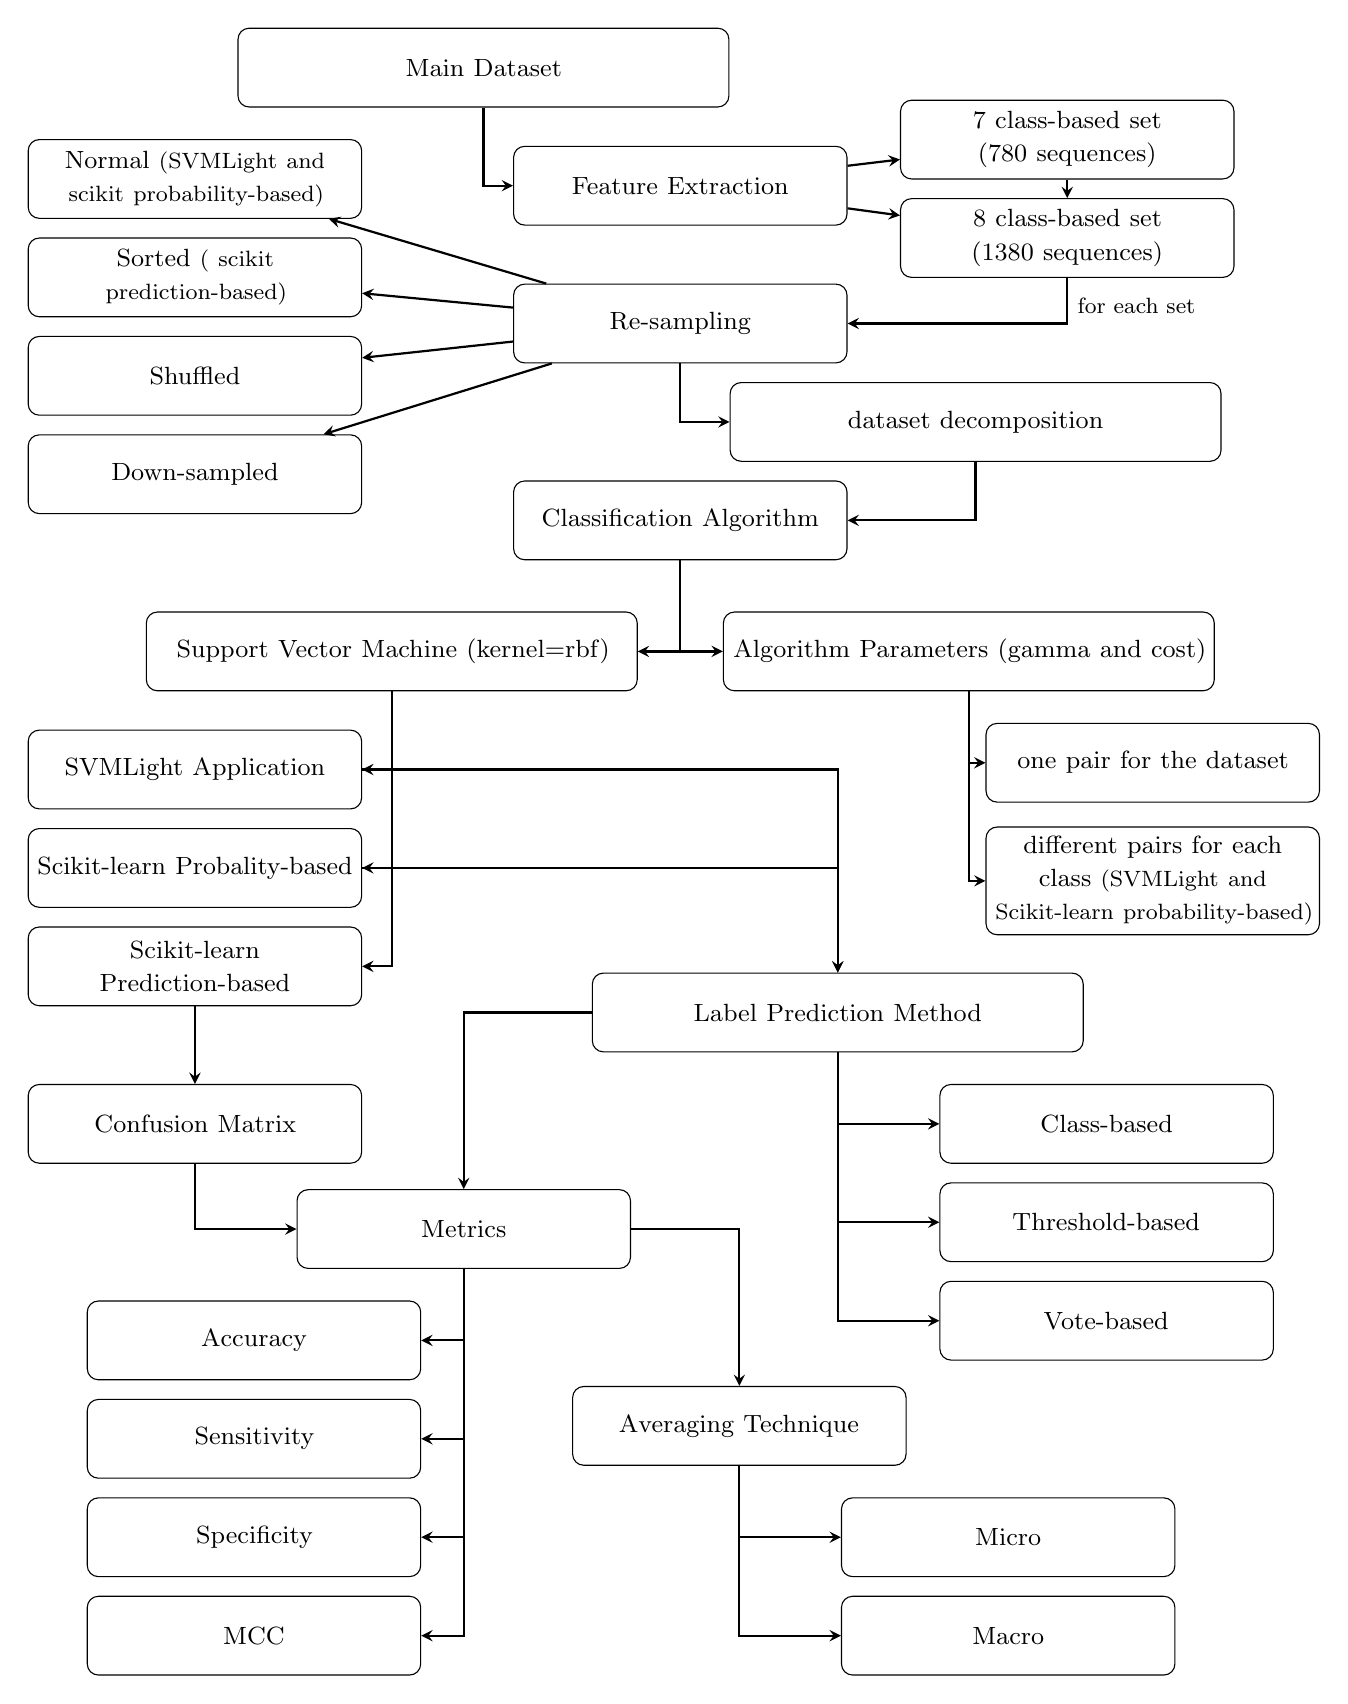
\begin{tikzpicture}[node distance=2cm]
    \node (dataset) [mainNode] {\small{Main Dataset}};
    \node (features) [branchNode, below of=dataset, yshift=0.5cm, xshift=2.5cm] {\small{Feature Extraction}};
    \node (7class) [branchNode, below right of=dataset, xshift= 6.0cm,yshift=0.5cm] {\small{7 class-based set (780 sequences)}};
    \node (8class) [branchNode, below of=7class,  yshift=0.75cm] {\small{8 class-based set (1380 sequences)}};
    % Resampling
    \node (resampling) [branchNode, below of=features, yshift=0.25cm, xshift=0cm] {\small{Re-sampling}};
    % Sorted, normal, down-sampled, shuffled
    \node (normal) [branchNode, below left of=dataset, xshift=-2.25cm, yshift=-0.0cm] {\small{Normal \footnotesize{(SVMLight and scikit probability-based)}}};
    \node (sorted) [branchNode, below of=normal, yshift=0.75cm] {\small{Sorted \footnotesize{( scikit prediction-based)}}};
    \node (shuffled) [branchNode, below of=sorted, yshift=0.75cm] {\small{Shuffled}};
    \node (downsampled) [branchNode, below of=shuffled, yshift=0.75cm] {\small{Down-sampled}};
    % Decomposition into binary problem
    \node (decomposition) [mainNode, below of=resampling, yshift=0.75cm, xshift=3.75cm] {\small{dataset decomposition}};
    % Algorithm
    \node (algorithm) [branchNode, below of=features, yshift=-2.25cm] {\small{Classification Algorithm}};
    % SVM, Parameters
    \node (svm) [mainNode, below left of=algorithm, xshift=-2.25cm, yshift=-0.25cm] {\small{Support Vector Machine (kernel=rbf)}};
    \node (parameters) [mainNode, below right of=algorithm, xshift=2.25cm, yshift=-0.25cm] {\small{Algorithm Parameters (gamma and cost)}};
    % svm=> SVMLight, Scikit-prediction, scikit-probability
    \node (svmLight) [branchNode, below of=svm, xshift=-2.5cm, yshift=0.5cm] {\small{SVMLight Application}};
    \node (scikitprob) [branchNode, below of=svmLight, yshift=0.75cm] {\small{Scikit-learn Probality-based}};
    \node (scikitpred) [branchNode, below of=scikitprob, yshift=0.75cm] {\small{Scikit-learn Prediction-based}};
    % Confusion Matrix
    \node (confusionMatrix) [branchNode, below of=scikitpred, yshift=0cm] {\small{Confusion Matrix}};
    % gamma and cost => one for each class, one for the whole dataset
    \node (onepair) [branchNode, below left of=parameters, xshift=3.75cm] {\small{one pair for the dataset}};
    \node (multiplepairs) [branchNode, below of=onepair, yshift=0.5cm] {\small{different pairs for each class 
     \footnotesize{(SVMLight and Scikit-learn probability-based)}}};
    %Prediction Methods
    \node (predMethods) [mainNode, below of=algorithm,  xshift=2cm, yshift=-4.25cm] {\small{Label Prediction Method}};
    %  class-based, threshold-based, vote-based
    \node (class) [branchNode, below right of=predMethods, xshift=2cm, yshift=0cm] {\small{Class-based}};
    \node (thereshold) [branchNode, below of=class, yshift=0.75cm] {\small{Threshold-based}};
    \node (vote) [branchNode, below of=thereshold, yshift=0.75cm] {\small{Vote-based}};
    % Metrics
    \node (metrics) [branchNode, below of=predMethods,  xshift=-4.75cm, yshift=-0.75cm] {\small{Metrics}};
    %  Sensitivity, Specificity, MCC, Accuracy
    \node (acc) [branchNode, below left of=metrics, xshift=-1.25cm, yshift=0] {\small{Accuracy}};
    \node (sens) [branchNode, below of=acc, yshift=0.75cm] {\small{Sensitivity}};
    \node (spec) [branchNode, below of=sens, yshift=0.75cm] {\small{Specificity}};
    \node (mcc) [branchNode, below of=spec, yshift=0.75cm] {\small{MCC}};
    %Averaging Techniques
    \node (avg) [branchNode, below of=metrics,  xshift=3.5cm, yshift=-0.5cm] {\small{Averaging Technique}};
    %  class-based, threshold-based, vote-based
    \node (micro) [branchNode, below right of=avg, xshift=2cm, yshift=0cm] {\small{Micro}};
    \node (macro) [branchNode, below of=micro, yshift=0.75cm] {\small{Macro}};

    \draw [arrow] (dataset) |- (features);
    \draw [arrow] (features) -- (7class);
    \draw [arrow] (features) -- (8class);
    % 
    \draw [arrow] (7class) -- (8class);
    \draw [arrow] (8class) |- node[anchor=south west] {\footnotesize{for each set}} (resampling);
    % 
    \draw [arrow] (resampling) -- (normal);
    \draw [arrow] (resampling) -- (sorted);
    \draw [arrow] (resampling) -- (shuffled);
    \draw [arrow] (resampling) -- (downsampled);
    % \draw [arrow] (8class) |- (algorithm);
    % 
    % \draw [arrow] (features) -- (resampling);
    \draw [arrow] (resampling) |- (decomposition);
    \draw [arrow] (decomposition) |- (algorithm);
    % 
    \draw [arrow] (algorithm) |- (svm);
    \draw [arrow] (algorithm) |- (parameters);
    % 
    \draw [arrow] (svm) |- (svmLight);
    \draw [arrow] (svm) |- (scikitpred);
    \draw [arrow] (svm) |- (scikitprob);
    % 
    \draw [arrow] (parameters) |- (onepair);
    \draw [arrow] (parameters) |- (multiplepairs);
    % 
    % \draw [arrow] (algorithm) -- (predMethods);
    \draw [arrow] (svmLight) -| (predMethods);
    \draw [arrow] (scikitprob) -| (predMethods);
    % 
    \draw [arrow] (scikitpred) -- (confusionMatrix);
    \draw [arrow] (confusionMatrix) |- (metrics);
    % 
    \draw [arrow] (predMethods) |- (class);
    \draw [arrow] (predMethods) |- (thereshold);
    \draw [arrow] (predMethods) |- (vote);
    %
    \draw [arrow] (predMethods) -| (metrics);
    \draw [arrow] (metrics) |- (acc);
    \draw [arrow] (metrics) |- (sens);
    \draw [arrow] (metrics) |- (spec);
    \draw [arrow] (metrics) |- (mcc);
    %
    \draw [arrow] (metrics) -| (avg);
    \draw [arrow] (avg) |- (micro);
    \draw [arrow] (avg) |- (macro);

\end{tikzpicture}
\end{adjustwidth}



\section*{Acknowledgments}


\nolinenumbers

% Either type in your references using
% \begin{thebibliography}{}
% \bibitem{}
% Text
% \end{thebibliography}
%
% or
%
% Compile your BiBTeX database using our plos2015.bst
% style file and paste the contents of your .bbl file
% here. See http://journals.plos.org/plosone/s/latex for 
% step-by-step instructions.
% 
\bibliographystyle{plos2015}
\bibliography{main.bib}


\end{document}

